\section{Rückwandlung innerer Energie}

\subsection{Zweiter Hauptsatz der Wärmelehre}

\begin{itemize}
	\item Innere Energie kann \textbf{nicht zu 100 \%} in Arbeit umgesetzt werden \\
		\textrightarrow\ Carnot-Wirkungsgrad ist der theoretisch höchstmögliche
	\item Wärme kann niemals \myul{von selbst} von einem kälteren Ort zu einem wärmeren Ort fliessen (Clausius)
	\item Es gibt keine \myul{periodisch wirkende} Maschine, die nichts anderes bewirkt als Erzeugung mechanischer Arbeit und 
		Abkühlung eines Wärme-Reservoirs (Kelvin) \\
		\textrightarrow\ Es gibt kein Perpetuum mobile 2. Art
\end{itemize}


\subsection{Kreisprozess (reversibler Prozess)}

\begin{center}
	Anfangszustand = Endzustand
\end{center}


\begin{minipage}[t]{0.48\columnwidth}
	\myul{\textbf{Rechts}laufender Kreisprozess}

	\smallskip

	\begin{itemize}
		\item Gibt Arbeit ab
		\item \cbl{Wärmekraftmaschine}
		\item Bei hoher Temperatur wird Wärme aus Prozess \textbf{zu}geführt
		\item Nur Bruchteil der Wärme in Arbeit verwandelbar
		\item Obergrenze: Carnot-Wirkungsgrad
	\end{itemize}
\end{minipage}
\hfill
\begin{minipage}[t]{0.48\columnwidth}
	\myul{\textbf{Links}laufender Kreisprozess}

	\smallskip

	\begin{itemize}
		\item Verbraucht Arbeit
		\item \cvt{Wärmepumpe}
		\item Bei hoher Temperatur wird dem Prozess Wärme \textbf{ab}geführt
		\item Erzeugt mehrfaches an Wärme
		\item Obergrenze: Inv. Carnot-Wirkungsgrad
	\end{itemize}
\end{minipage}

\subsection{Carnot-Wirkungsgrad}

\vspace{-0.2cm}

$$ \boxed{\text{\cbl{Wärmekraftmaschine:}}  \quad \eta_C = \frac{W_{\rm ab}}{Q_{\rm zu}} = \frac{T_{\rm hoch} - T_{\rm tief}}{T_{\rm hoch}} } $$

$$ \boxed{\text{ \cvt{Wärmepumpe:}} \quad  \eta_{iC} = \frac{Q_{\rm zu}}{W_{\rm ab}} = \frac{T_{\rm hoch}}{T_{\rm hoch} - T_{\rm tief}} } $$


\begin{tabular}{c l c}
	$n_C$ 			& Carnot-Wirkungsgrad 				& $[n_C] = 1$ 					\\
	$n_{iC}$ 		& Inverset Carnot-Wirkungsgrad 		& $[n_{iC}] = 1$ 				\\
	$T_{\rm tief}$ 	& Temperatur des Warm-Reservoirs 	& $[T_{\rm tief}] = \kelvin$	\\
	$T_{\rm hoch}$ 	& Temperatur des Kalt-Reservoirs 	& $[T_{\rm hoch}] = \kelvin$ 	\\
	$Q_{\rm zu}$ 	& zugeführte Wärme 					& $[Q_{\rm zu}] = \joule$ 		\\ 
	$W_{\rm ab}$ 	& abgeführte Energie 				& $[W_{\rm ab}] = \joule$
\end{tabular}

\subsubsection{Molare Wärmekapazität von Gasen}

$$\boxed{C_{mp} - C_{mV} = R} $$

\renewcommand{\arraystretch}{1.3}
\begin{tabular}{c l l}
	$C_{mp}$ 	& Isobare Wärme-Kapazität $(p = \const)$ 									& $[C_{mp}] = \frac{\joule}{\mole \, \kelvin}$	\\
	$C_{mV}$ 	& Isochore Wärme-Kapazität $(V = \const)$ 									& $[C_{mV}] = \frac{\joule}{\mole \, \kelvin}$	\\
\end{tabular}
\renewcommand{\arraystretch}{1}

\renewcommand{\arraystretch}{1.4}
\begin{center}
	\begin{tabular}{|l|c|c|}
		\hline
		& $\Delta W$ 			& $\Delta Q$ 		\\
		& {\tiny abgeführte Arbeit} 	& {\tiny zugeführte Wärme}	\\
		\hline
		$\Delta p = 0$: Isobar 	& $p(V_2-V_1)$			& $nC_{mp}(T_2-T_1)$\\
		\hline
		$\Delta V = 0$: Isochor	& $0$					& $nC_{mV}(T_2-T_1)$	\\
		\hline
		$\Delta T = 0$: Isotherm	& $nRT \cdot ln(\frac{V_2}{V_1})$& $nRT \cdot ln(\frac{V_2}{V_1})$		\\
		\hline
		$\Delta Q = 0$: adiabatisch & $-nC_{mv}(T_2-T_1)$& $0$				\\
		\hline	
	\end{tabular}
\end{center}
\renewcommand{\arraystretch}{1}

\subsection{Kreisprozesse (Vorgänge)}

\begin{tabular}{lll}
	isotherme Expansion 		& liefert Wärme 	& benötigt Energie	\\
	isotherme Kompression 		& benötigt Wärme 	& liefert Energie 	\\
	\\
	adiabatische Expansion 		& liefert Arbeit 	& ohne Wärme 		\\
	adiabatische Kompression 	& benötigt Arbeit 	& ohne Wärme 		\\
	\\
	isochore Erwärmung 			& ohne Arbeit 		& benötigt Wärme 	\\
	isochore Abkühlung 			& ohne Arbeit 		& liefert Wärme
\end{tabular}

\begin{minipage}[c]{0.48\columnwidth}
	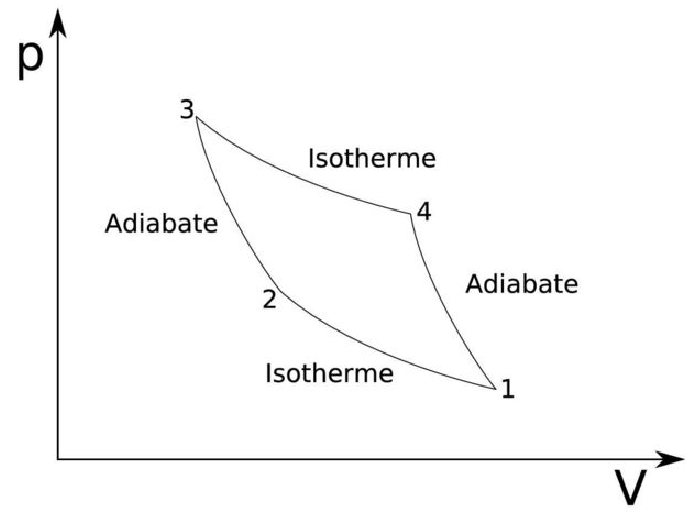
\includegraphics[width=\columnwidth]{images/kreisprozess_2.png}
\end{minipage}
\hfill
\begin{minipage}[c]{0.48\columnwidth}
	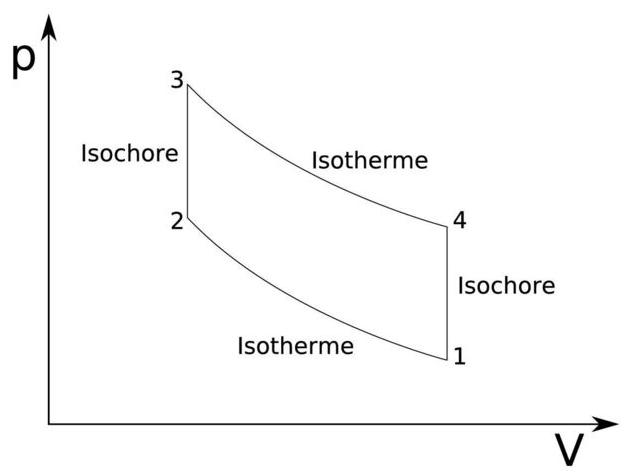
\includegraphics[width=\columnwidth]{images/kreisprozess_3.png}
\end{minipage}

\begin{center}
	\begin{tabular}{l l l}
		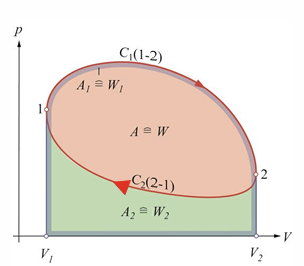
\includegraphics{images/Kreisprozess_4.png}	& & 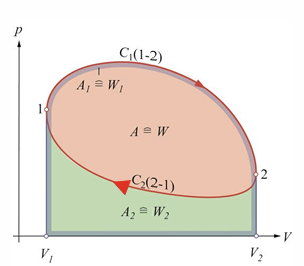
\includegraphics{images/Kreisprozess_4.png} \\
		\textbf{Rechtslaufender Kreisprozess}	& &\textbf{Linkslaufender Kreisprozess}	\\
		- gibt das System Arbeit ab		& &- gibt Wärme ab				\\
		- dem System wird Wärme zugeführt & &- dem System wird Arbeit zugeführt	\\
		\textbf{Wärmekraftmaschine}		& &\textbf{Wärmepumpe / Kältemaschine} 
	\end{tabular}
\end{center}

\pagebreak

